
\documentclass[a4paper,12pt]{article}
%%%%%%%%%%%%%%%%%%%%%%%%%%%%%%%%%%%%%%%%%%%%%%%%%%%%%%%%%%%%%%%%%%%%%%%%%%%%%%%%%%%%%%%%%%%%%%%%%%%%%%%%%%%%%%%%%%%%%%%%%%%%%%%%%%%%%%%%%%%%%%%%%%%%%%%%%%%%%%%%%%%%%%%%%%%%%%%%%%%%%%%%%%%%%%%%%%%%%%%%%%%%%%%%%%%%%%%%%%%%%%%%%%%%%%%%%%%%%%%%%%%%%%%%%%%%
\usepackage{eurosym}
\usepackage{vmargin}
\usepackage{amsmath}
\usepackage{graphics}
\usepackage{epsfig}
\usepackage{subfigure}
\usepackage{fancyhdr}

\setcounter{MaxMatrixCols}{10}
%TCIDATA{OutputFilter=LATEX.DLL}
%TCIDATA{Version=5.00.0.2570}
%TCIDATA{<META NAME="SaveForMode"CONTENT="1">}
%TCIDATA{LastRevised=Wednesday, February 23, 201113:24:34}
%TCIDATA{<META NAME="GraphicsSave" CONTENT="32">}
%TCIDATA{Language=American English}

\pagestyle{fancy}
\setmarginsrb{20mm}{0mm}{20mm}{25mm}{12mm}{11mm}{0mm}{11mm}
\lhead{MA4128} \rhead{Kevin O'Brien} \chead{Cluster Analysis  } %\input{tcilatex}

\begin{document}

\section{Clustering Algorithm}
To better understand how a clustering algorithm works, let’s manually examine
some of the single linkage procedure’s calculation steps. We start off by looking at
the initial (Euclidean) distance matrix displayed previously.

\begin{figure}[h!]
	\begin{center}
		% Requires \usepackage{graphicx}
		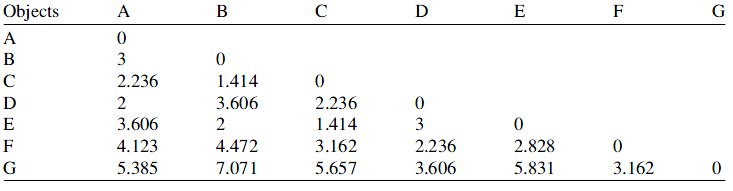
\includegraphics[scale=0.6]{images/DistanceMatrix.jpg}\\
	\end{center}
\end{figure}



\begin{itemize}
	\item In the very first step, the two
	objects exhibiting the smallest distance in the matrix are merged. Note that we
	always merge those objects with the smallest distance, regardless of the clustering
	procedure (e.g., single or complete linkage). (N.B. In the following example, ties will be broken at random.)
	\item As we can see, this happens to two
	pairs of objects, namely B and C (d(B, C) = 1.414), as well as C and E (d(C, E) =
	1.414). In the next step, we will see that it does not make any difference whether we
	first merge the one or the other, so let’s proceed by forming a new cluster, using
	objects B and C.
	\begin{figure}[h!]
		\begin{center}
			% Requires \usepackage{graphicx}
			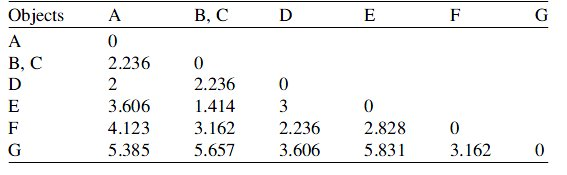
\includegraphics[scale=0.6]{images/DistanceMatrix2.jpg}\\
		\end{center}
	\end{figure}
	\item Having made this decision, we then form a new distance matrix by considering
	the single linkage decision rule as discussed above. According to this rule, the
	distance from, for example, object A to the newly formed cluster is the minimum of
	$d(A, B)$ and $d(A, C)$. As $d(A, C)$ is smaller than d(A, B), the distance from A to the
	newly formed cluster is equal to d(A, C); that is, 2.236.
	\item We also compute the
	distances from cluster [B,C] (clusters are indicated by means of squared brackets)
	to all other objects (i.e. D, E, F, G) and simply copy the remaining distances – such
	as $d(E, F)$ – that the previous clustering has not affected.
	\begin{figure}[h!]
		\begin{center}
			% Requires \usepackage{graphicx}
			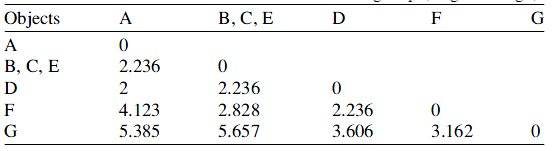
\includegraphics[scale=0.6]{images/DistanceMatrix3.jpg}\\
		\end{center}
	\end{figure}
	\item Continuing the clustering procedure, we simply repeat the last step by merging
	the objects in the new distance matrix that exhibit the smallest distance (in this case,
	the newly formed cluster [B, C] and object E) and calculate the distance from this
	cluster to all other objects.
	\begin{figure}[h!]
		\begin{center}
			% Requires \usepackage{graphicx}
			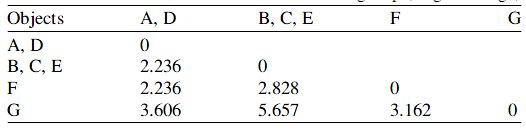
\includegraphics[scale=0.6]{images/DistanceMatrix4.jpg}\\
		\end{center}
	\end{figure}
	\item We continue in the same fashion until one cluster is left. By following the single linkage procedure, the last steps involve the merger
	of cluster [A,B,C,D,E,F] and object G at a distance of 3.162.
	\begin{figure}[h!]
		\begin{center}
			% Requires \usepackage{graphicx}
			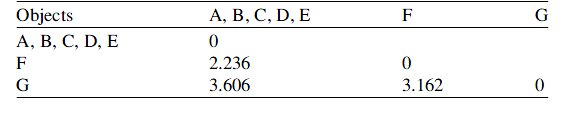
\includegraphics[scale=0.6]{images/DistanceMatrix5.jpg}\\
		\end{center}
	\end{figure}
	\begin{figure}[h!]
		\begin{center}
			% Requires \usepackage{graphicx}
			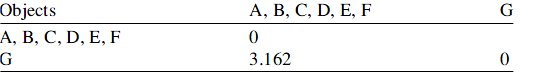
\includegraphics[scale=0.6]{images/DistanceMatrix6.jpg}\\
		\end{center}
	\end{figure}
\end{itemize}
\newpage







\section{Clustering Algorithm}
To better understand how a clustering algorithm works, let’s manually examine
some of the single linkage procedure’s calculation steps. We start off by looking at
the initial (Euclidean) distance matrix displayed previously.

\begin{figure}[h!]
	\begin{center}
		% Requires \usepackage{graphicx}
		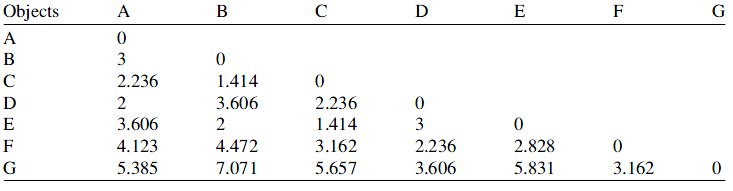
\includegraphics[scale=0.6]{images/DistanceMatrix.jpg}\\
	\end{center}
\end{figure}

\begin{itemize}
	\item In the very first step, the two
	objects exhibiting the smallest distance in the matrix are merged. Note that we
	always merge those objects with the smallest distance, regardless of the clustering
	procedure (e.g., single or complete linkage). (N.B. In the following example, ties will be broken at random.)
	\item As we can see, this happens to two
	pairs of objects, namely B and C (d(B, C) = 1.414), as well as C and E (d(C, E) =
	1.414). In the next step, we will see that it does not make any difference whether we
	first merge the one or the other, so let’s proceed by forming a new cluster, using
	objects B and C.
	\begin{figure}[h!]
		\begin{center}
			% Requires \usepackage{graphicx}
			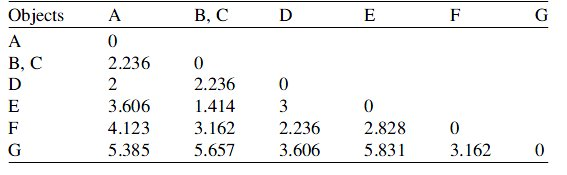
\includegraphics[scale=0.6]{images/DistanceMatrix2.jpg}\\
		\end{center}
	\end{figure}
	\item Having made this decision, we then form a new distance matrix by considering
	the single linkage decision rule as discussed above. According to this rule, the
	distance from, for example, object A to the newly formed cluster is the minimum of
	d(A, B) and d(A, C). As d(A, C) is smaller than d(A, B), the distance from A to the
	newly formed cluster is equal to d(A, C); that is, 2.236.
	\item We also compute the
	distances from cluster [B,C] (clusters are indicated by means of squared brackets)
	to all other objects (i.e. D, E, F, G) and simply copy the remaining distances – such
	as d(E, F) – that the previous clustering has not affected.
	\begin{figure}[h!]
		\begin{center}
			% Requires \usepackage{graphicx}
			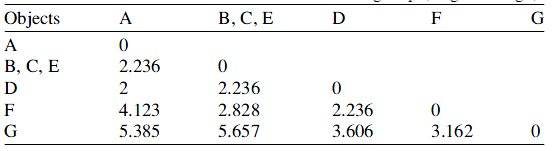
\includegraphics[scale=0.6]{images/DistanceMatrix3.jpg}\\
		\end{center}
	\end{figure}
	\item Continuing the clustering procedure, we simply repeat the last step by merging
	the objects in the new distance matrix that exhibit the smallest distance (in this case,
	the newly formed cluster [B, C] and object E) and calculate the distance from this
	cluster to all other objects.
	\begin{figure}[h!]
		\begin{center}
			% Requires \usepackage{graphicx}
			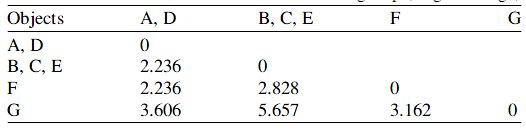
\includegraphics[scale=0.6]{images/DistanceMatrix4.jpg}\\
		\end{center}
	\end{figure}
	\item We continue in the same fashion until one cluster is left. By following the single linkage procedure, the last steps involve the merger
	of cluster [A,B,C,D,E,F] and object G at a distance of 3.162.
	\begin{figure}[h!]
		\begin{center}
			% Requires \usepackage{graphicx}
			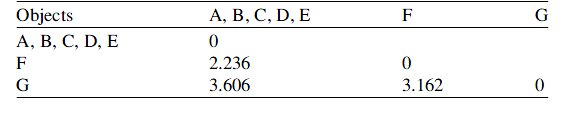
\includegraphics[scale=0.6]{images/DistanceMatrix5.jpg}\\
		\end{center}
	\end{figure}
	\begin{figure}[h!]
		\begin{center}
			% Requires \usepackage{graphicx}
			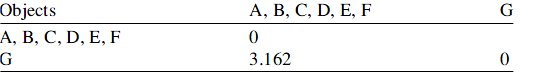
\includegraphics[scale=0.6]{images/DistanceMatrix6.jpg}\\
		\end{center}
	\end{figure}
\end{itemize}
\end{document}

